%chktex-file 36
%chktex-file 23
%chktex-file 10
%chktex-file 17
%chktex-file 9
\documentclass[ComputationalMathematics.tex]{subfiles}

\begin{document}

%%%%%%%%%%%%%%~~~~~~~~~~~~~~~~~~~~~~~~~~~~~~~~~~~~~~~~%%%%%%%%%%%%%%%
\section{5th of October 2018 --- A. Frangioni}
%%%%%%%%%%%%%%~~~~~~~~~~~~~~~~~~~~~~~~~~~~~~~~~~~~~~~~%%%%%%%%%%%%%%%
\subsection{Unconstrained optimization}

Until now we stated that the best conditions are encountered when the domain is a compact set and we have many derivatives.

Now we need to consider when we can stop our algorithm.

\begin{definition}[Unconstrained optimization problem]
We want to solve:
\[
  f_* = \min \{f(x)~:~x \in X\}~(P)
\]

where $X = \R^n$.
\end{definition}

If $\R^n$ is not bounded, Weierstrass theorem does not apply, hence even if a (global) minimum $x_*$ exists, finding it is a NP problem.

Let us use a weaker condition to ease things a little: $x_*$ is a \textbf{local minimum} if it solves:
\[
  \min \{f(x)~:~x \in \mathcal{B}(x_*, \eps) \}\mbox{for some } \eps > 0
\]
aka, the minimum we found is a global minimum in a ball around $x^*$.

Also, $x^*$ is a \textbf{strict local minimum} if $f(x) \,  {<} \, f(y) \;\; \forall \, y \in \mathcal{B}( \, x_* \,,\, \eps \, )$

To test these conditions derivatives help, as an example see \Cref{fig:5ott_1}


\begin{figure}[h]
  \centering
  \subfloat[][Not minima]{\includegraphics[width=0.35\textwidth]{pics/5ott/localopt1.pdf}\label{subfloat:5ott_1}}
  \hspace{0.5cm}
  \subfloat[][Minima]{\includegraphics[width=0.35\textwidth]{pics/5ott/localopt2.pdf}\label{subfloat:5ott_2}}\\
  \caption{In the leftmost plot, we can see that if the derivatives are non zero the point is not a minimum. Such a condition is satisfied in the right handed plot.}\label{fig:5ott_1}
\end{figure}

If $f'(x) < 0$ or $f'(x) > 0$, $x$ clearly cannot be a local minimum.
 
Hence, $f'(x) = 0$ in all local minima, so this holds in the global one as well.

\subsubsection{First order model}
\recap{The first order model of $f$ is $L_x(y) = f(x) + \nabla f(x) (y-x)$, such that $f(y) = f(x) + \nabla f(x) (y-x) + R(y-x)$.

We already stated last lecture that if the norm of the argument of the residual is going to $0$, then the residual is going to $0$ faster (quadratically), formally $\lim\limits_{\norm{h} \to 0} \frac{R(h)}{\norm{h}} = 0$.}

\begin{proposition}
Let $f$ be differentiable, if $x$ is a local minimum, then $\nabla f(x) = 0$.
\end{proposition}

In which direction shall we move in order to get closer to the minimum, provided that we are sitting in $x$?
$x(\alpha) = x - \alpha \nabla f(x)$, hence we should take a step along the anti-gradient $- \nabla f(x)$.

\begin{proof}[Proof by contraddiction]
  Let us assume that $x$ is a local minimum but $\nabla f(x) \neq 0$.
  
  In our case, $y = x -\alpha \nabla f(x)$, so we get $f(x - \alpha \nabla f(x)) = f(x) - \alpha \norm{\nabla f(x)}^2 + R(- \alpha \nabla f(x))$.

Hence, in our case the direction is fixed, but we can choose the step size $\alpha$, so it can be proved that $\lim\limits_{\alpha \to 0} \frac{R(- \alpha \nabla f(x))}{\norm{\alpha \nabla f(x)}} = 0$, that is equivalent by definition to $\forall \eps > 0 \, \exists \bar{\alpha} > 0$ s.t. $\frac{R(- \alpha \nabla f(x))}{\alpha \norm{\nabla f(x)}} \leq \eps~\forall ~ 0 \leq \alpha < \bar{\alpha}$.

  Take $\eps < \norm{nabla f(x)}$ to get  $R(- \alpha \nabla f(x)) < \alpha \norm{\nabla f(x)}^2$, then 
\[
  f(x(\alpha)) = f(x) - \alpha \norm{\nabla f(x)}^2 + R(- \alpha \nabla f(x)) < f(x)
\]
$\forall \alpha < \bar{\alpha}~x$ cannot be a local minimum.
\end{proof}

Notice that the optimality condition also tells us how to move to get closer to the minimum.

An attentive reader may notice that the gradient is $0$ in minima, maxima and saddle points (aka stationary point), hence how to discriminate among those?


We need to take infot account second derivatives, namely such second derivative should be positive for a minimum point.

\subsubsection{Second order model}

\begin{proposition}
Let $f \in C^2$. If $x$ is a local minimum then $\nabla^2 f(x) \succeq 0$, in words the gradient is positive semidefinite.
\end{proposition}

\begin{proof}[Proof by contraddiction]
  Our contraddictory hypothesis is that we are in a local minimum, but the Hessian is not positive semidefinite (formally, $\exists d$ s.t.~$d^T \nabla^2 f(x) d < 0$ or equivalently, $\exists \lambda_i <0$, noticing that $\bar{f}(\alpha)  = tr{(\alpha H_i)} \nabla f(x) (\alpha H_i) = \alpha^2 \lambda_i < 0$).
  
  Obs: saying that Hessian is not positive semidefinite means saying that there is a direction of negative curvature.

  Just like in previous case, we take the direction $d$ normalized ($\norm{d} = 1$).

  Let us consider a step $x(\alpha) = x + \alpha d$ and then take the second-order Taylor formula (since $\nabla f(x) = 0$ there is no linear term involved)
\[
  f(x(\alpha)) = f(x) + \frac{1}{2} \alpha^2 d^T \nabla^2 f(x) d + R( \alpha d )
\]
with $\lim\limits_{\norm{h} \to 0} \frac{R(h)}{\norm{h}^2} = 0$, which means that the residual should go to $0$ at least cubically.
  
Since $h = x - x(\alpha)$ we get that $\lim\limits_{\alpha \to 0} \frac{R(\alpha d)}{\alpha^2} = 0$ or equivalently $\forall \eps > 0 \, \exists \bar{\alpha} > 0$ s.t. $R(\alpha d) \leq \eps \alpha^2 \forall 0 \leq \alpha < \bar{\alpha}$.

At this point, since this condition holds for each $\epsilon$ we are allowed to take the most convenient: $\eps < -\frac{1}{2} d^T \nabla^2 f(x) d$, so that we obtain this condition on the residual $R(\alpha d) < -\frac{1}{2} \alpha^2 d^T \nabla^2 f(x) d$, hence
\[
f(x(\alpha)) = f(x) + \frac{1}{2} \alpha^2 d^T \nabla^2 f(x) d + R(\alpha d) < f(x) \forall \, 0 \leq \alpha < \bar{\alpha}
\]
Hence $x$ cannot be a local minimum.
\end{proof}


  In a local minimum, there cannot be directions of  negative curvature ``when the first derivative is $0$, second-order effects prevail''.

As far as sufficient conditions are concerned, we can prove the following

\begin{proposition}
  Let $f \in C^2$ and let the Hessian be symmetric (hence real eigenvalues).
  If $\nabla f(x) = 0$ and the Hessian is strictly positive definite ($\nabla^2 f(x) \succ 0$) then $x$ is a local minimum.
\end{proposition}

\begin{proof}
Since the gradient is $0$ we get the following second order Taylor approximation
\[
  f(x + d) = f(x) + \frac{1}{2} d^T \nabla^2 f(x) d + R(d)\mbox{ with } \lim\limits_{h \to 0} \frac{R(d)}{\norm{d}^2} = 0
\]
  Hence, by definition of limit $\forall \eps > 0~\exists~\delta > 0$ s.t. $R(d) \leq \eps \norm{d}^2~\forall d$ s.t. $\norm{d} < \delta$.

Since the Hessian is strictly positive definite $\lambda_{\text{min}} > 0$ minimum eigenvalue of $\nabla^2 f(x)$, hence the variational caracterization of eigenvalues $d^T \nabla^2 f(x) d \geq \lambda_{\text{min}} \norm{d}^2$.

  We are now ready to pick the $\eps$ we prefer ($\eps < \lambda_{\text{min}}$) to get $\forall d$ s.t. $\norm{d} < \delta$
\[
  f(x + d) = f(x) + \frac{1}{2} d^T \nabla^2 f(x) d + R(d) \geq f(x) + (\lambda_{\text{min}} - \eps)\|d\|^2 > f(x)
\]

  The term $\lambda_{\text{min}} - \eps$ is strictly positive
\end{proof}

In the remaining part of this lecture we will look for conditions that ensure that one a local minimum is found, it is also a global minimum.

Until now, we said that the local minima are those points where the gradient is $0$ and the Hessian is positive semidefinite.
An easy way to ensure that the Hessian is positive semidefinite in a ball around $x$ is to have that the Hessian is positive semidefinite everywhere ($\forall x \in \R^n$) aka $f$ is a convex function.

\subsection{Convexity}
Let us introduce some preliminaries to the hypothesis of convex functions.

\begin{definition}[Convex hull]
  Let $x, y \in \R^n$ we term \textbf{convex hull} and denote conv$(x, y) = \{z = \alpha x + ( 1 - \alpha ) y~:~ \alpha \in [0, 1]\}$ the segment joining $x$ and $y$.
\end{definition}

\begin{definition}[Convex set]
  We term \textbf{convex set} if for each couple in the set, the line linksing such points belongs to the set.

  Formally, $C \subset \R^n$ is a \textbf{convex set} if $\forall~x, y \in C$ conv$(x,y) \subseteq C$.
\end{definition}

Notice that ``disconnected sets'' cannot be convex sets.

\begin{definition}[Convex hull of a set]
Given a set $S$, we can ``complete'' it to a convex set:
\[
\begin{array}{rcl}
 conv(S) & = &
 \bigcup \{ \, conv(x,y) \,:\, x, y \in S \, \} \\[0.2cm]
 & = &
 \bigcap \{ \, C \,:\, C \mbox{ is convex } \wedge
                         C \supseteq S \, \}
\end{array}
\]
Equivalently, the convex hull of $S$ = iterated convex hull of all $x, y \in S$ or the smallest convex set containing $S$
\end{definition}

Our goal is to find the nicest possible convex set that approximates our set.

\begin{proposition}
A convex set is equal to its convex hull, formally $C$ is convex $\iff C = conv(C)$.
\end{proposition}

\begin{myframe}{\bf Note}
A more general definition of a convex hull is the following:
conv$(\{x_1, \ldots, x_k\}) = \{x = \sum_{i=1}^k \alpha_i x_i~:~\sum_{i=1}^k \alpha_i = 1,~\alpha_i \geq 0~\forall i\}$ 
\end{myframe}

\begin{definition}[Unitary simplex]
  We term \textbf{unitary simplex} the set of $k$ non-negative numbers summing to $1$, formally
\[
\Theta^k = \{\alpha_i \in \R^k~:~\sum_{i=1}^k \alpha_i = 1, \alpha_i \geq 0~\forall i\}
\]

  A few graphical examples are displayed in \Cref{fig:5ott_2}.
\end{definition}

\begin{figure}[h]
  \centering
  \subfloat[][In $\R^2$]{\includegraphics[width=0.35\textwidth]{pics/5ott/usR2.png}\label{subfloat:5ott_3}}
  \hspace{0.5cm}
  \subfloat[][In $\R^3$]{\includegraphics[width=0.35\textwidth]{pics/5ott/usR3.png}\label{subfloat:5ott_4}}\\
  \caption{Unitary simplexes.}\label{fig:5ott_2}
\end{figure}


We are interested in sufficient conditions for convexity.

\begin{definition}[Cone]
  We term \textbf{cone} the set $\mathcal{C} = \{x~:~\alpha x \in \mathcal{C}\forall\alpha \geq 0\}$.
\end{definition}

An attentive reader may notice that the definition of cone is a relaxation of the unitary simplex, where we do not require the unitary sum.

The following sets are convex:
\begin{itemize}
  \item Convex polytope $conv( \, \{x_1, \ldots, x_k\} \, )$, unitary simplex $\Theta$
  \item Affine hyperplane: $\mathcal{H} := \{x \in \R^n~:~ax = b\}$
  \item Affine subspace: $\mathcal{S} := \{x \in \R^n~:~ ax \leq b\}$
  \item Ball in $p$-norm, $p \geq 1$: $\mathcal{B}_p( \, x \,,\, r \, ) = \{ \, y \in \R^n \,:\, \| \, y - x \, \|_p \leq r \,\}$
  \item Ellipsoid: $\mathcal{E}(Q,x,r) := \{y \in \R^n~:~\tr{(y - x)}Q(y - x) \leq r\}$  with $Q \succeq 0$. Notice that ellipsoids are levelsets of quadratic functions.
  \item Open versions by substituting ``$<$'' to ``$\leq$''
  \item Cones
  \item Conical hull of a finite set of directions: $cone(\{d_1, \ldots, d_k\}) = \Big\{ \, d = \sum\limits_{i=1}^k \mu_i d_i~:~\mu_i \geq 0~\forall \, i \, \Big\}$
  \item Lorentz (ice-cream) cone: $\mathbb{L} = \Big\{ \, x \in \R^n \,:\, x_n \geq \sqrt{\sum_{i=1}^{n-1} x_i^2} \, \Big\}$
  \item Cone of positive semidefinite matrices: $\mathbb{S}_+ = \{ \, A \in \R^{n \times n} \,:\, A \succeq 0\}$
\end{itemize}

\begin{proposition}
The following operations preserve convexity.
\begin{enumerate}
  \item Given a possibly infinite family of convex sets (${\{C_i\}}_{i \in I}$), the intersection ($\bigcap_{i \in I} C_i$) convex;
  
  \item If we have convex sets in different subspaces, their cartesian product is a convex set ($C_1, \ldots, C_k$ convex $\iff C_1 \times \cdots \times C_k$ convex);
  
  \item Given a convex set, its image under a linear mapping (aka scaling, translation, rotation) is a convex set. Formally, $C$ convex $\Longrightarrow A(C) := \{x = Ay + b~:~y \in C\}$ convex; 
  
  \item $C$ convex $\Longrightarrow A^{-1}(C) := \{x~:~Ax + b \in C\}$ convex (inverse image under a linear mapping);
  
  \item Let $C_1$ and $C_2$ convex and let $\alpha_1, \alpha_2 \in \R$. Then $\alpha_1 C_1 + \alpha_2 C_2 := \{ x = \alpha_1 x_1 + \alpha_2 x_2 \,:\, x_1 \in C_1, x_2 \in C_2\}$ convex;
  \item $C \subseteq \R^n = \R^{n_1} \times \R^{n_2}$ convex $\Longrightarrow$
  \begin{description}
    \item[{\small \sc Slice:}] $C(y) := \{x \in \R^{n_1}~:~(x, y) \in C\}$ convex;
    \item[{\small \sc Projection:}] $C^1 := \{x \in \R^{n_1}~:~\exists y$ s.t. $(x, y) \in C\}$ convex
  \end{description}
    A pictorial example in \Cref{fig:5ott_3};
  \item $C$ convex $\Longrightarrow int(C)$ and $cl(C)$ convex
\end{enumerate}
\end{proposition}

\begin{figure}[h]
  \centering
  \subfloat[][Slice on $\bar{y}$]{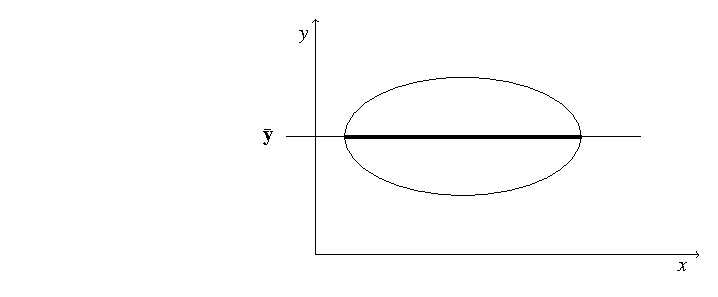
\includegraphics[width=0.35\textwidth]{pics/5ott/slice.png}\label{subfloat:5ott_5}}
  \hspace{0.5cm}
  \subfloat[][Project on the $x$ component]{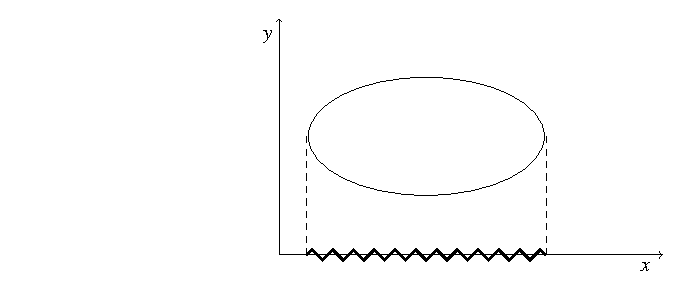
\includegraphics[width=0.35\textwidth]{pics/5ott/project.png}\label{subfloat:5ott_6}}\\
  \caption{Pictorial examples of slicing and projecting.}\label{fig:5ott_3}
\end{figure}

\begin{theorem}
  $\mathcal{P}$ is a polyhedron iff $\exists \{x_1, \ldots, x_k\}$ and $\{d_1, \ldots, d_h\}$ s.t. $\mathcal{P} = conv(\{x_1, \ldots, x_k\}) + \text{cone}(\{d_1, \ldots, d_h\})$.
\end{theorem}

Notice that if we are interested in proving that a set with a certain shape is convex, we chould try to derive it from an object that we know is convex through the operations we enumerated above.

\begin{definition}[Convex function]
  Let $f:\R^n \to \R^m$ be a function. We say that $f$ is \textbf{convex} if $\forall x, y \in \R^n$, the segment that joins $f(x)$ and $f(y)$ lies above the function.

  In other words, $f$ is \textbf{convex} iff $epi(f)$ is convex, where $epi$ denotes the epigraph of the function, graphically speaking, the region which is above the function line (in the plot).

  Equivalently, we say that $f$ is \textbf{convex} if $\forall x, y \in dom(f)$ for any $\alpha \in [0, 1]$, $\alpha f(x) + (1-\alpha) f(y) \geq f(\alpha x + (1-\alpha)y)$.

  Equivalently, $\forall x^1$, \ldots, $x^k$, $\alpha \in \Theta^k$
\[
 f \left( \sum_{i=1}^k \alpha_i x^i \right) \leq \sum_{i=1}^k \alpha_i f(x^i)
\]
\end{definition}

\begin{definition}[Sublevel graph]
  Let $f: \R^n \to \R^m$ be a function. We term \textbf{sublevel graph} of $f(x)$ the projection on the $x$ axis of the portions of the epigraph which lie below the constant $y=\bar{x}$.
\end{definition}

\addpic{0.7}{pics/5ott/sub.png}{Pictorial example of sublevel graph. Such a graph is drawn in green in the figure.}{fig:5ott_4}

\begin{proposition}\label{prop:5ott_1}
The following holds:
\begin{itemize}
 \item Let $f$ convex. Then $S(f,v)$ convex $\forall v \in \R$;
 \item $f$ is concave if $-f$ is convex (``convex analysis is a one-sided world'').
\end{itemize}
\end{proposition}

The second statement of \Cref{prop:5ott_1} is useful to make a comparison between minimizing and maximizing. In particular, if our aim is to maximize the function, we can be sure to have found a global maximum if the function is concave.

\begin{definition}[Strict convexity]
  Let $f: \R^n \to \R^m$. We term $f$ \textbf{strictly convex} iff $\alpha f(x) + (1 - \alpha) f(y) > f(\alpha x + (1 - \alpha) y )$.
\end{definition}


\begin{definition}[Strong convexity]
  Let $f: \R^n \to \R^m$. We term $f$ \textbf{strongly convex modulus $\tau > 0$} iff $f(x) - \frac{\tau}{2}\,\norm{x}^2$ is convex.
  
  Formally,
 \[
   \alpha f(x) + (1 - \alpha) f(y) \geq f(\alpha x + (1 - \alpha) y)+ \frac{\tau}{2} \alpha (1 - \alpha) \norm{(y - x)}^2
 \]
\end{definition}

Next lecture we will talk about how we can check tat a function is convex, operationally.
\end{document}
